
\documentclass[11pt,border=3pt]{standalone}
\pdfcompresslevel=0\pdfobjcompresslevel=0 
%\usepackage[letterpaper]{geometry}
% amsmath package, useful for mathematical formulas
\usepackage{amsmath}
% amssymb package, useful for mathematical symbols
\usepackage{amssymb}
\usepackage{tikz}
\usepackage{graphicx}
\usepackage{relsize}
\usepackage{mathptmx}
\usetikzlibrary{matrix,positioning,arrows,fit,shapes,shadows,snakes,shadows}

% graphicx package, useful for including eps and pdf graphics
\usepackage{graphics,graphicx}

% Generate the pdf: latex Figure1;dvips Figure1.dvi;ps2epsi Figure1.ps;epspdf Figure1.epsi

%!TEX root = main_RNAPyro_JCB.tex

\newcommand{\ourprog}{\texttt{RNA-MoIP}\xspace} 

\usepackage[applemac]{inputenc} %for the encoding 


\newcommand{\RNAmutants}{\texttt{RNAmutants}\xspace}
\newcommand{\RNApyro}{\texttt{RNApyro}\xspace}

\newcommand{\red}[1]{{\color{red}#1}}
\newcommand{\farna}{\texttt{FARNA}\xspace}
\newcommand{\mcfoldmcsym}{\texttt{MC-Pipeline}\xspace}
\newcommand{\mcfold}{\texttt{MC-Fold}\xspace}
\newcommand{\mcsym}{\texttt{MC-Sym}\xspace}
\newcommand{\nast}{\texttt{NAST}\xspace}
\newcommand{\ifoldrna}{\texttt{iFoldRNA}\xspace}
\newcommand{\rnafold}{\texttt{RNAfold}\xspace}
\newcommand{\rnasubopt}{\texttt{RNAsubopt}\xspace}
\newcommand{\rnawolf}{\texttt{RNAwolf}\xspace}
\newcommand{\rnastructure}{\texttt{RNAstructure}\xspace}
\newcommand{\contrafold}{\texttt{contrafold}\xspace}
\newcommand{\unafold}{\texttt{unafold}\xspace}
\newcommand{\rnadd}{\texttt{RNA2D3D}\xspace}
\newcommand{\assemble}{\texttt{assemble}\xspace}
\newcommand{\fred}{\texttt{FR3D}\xspace}
\newcommand{\rnajunction}{\texttt{RNAjunction}\xspace}
\newcommand{\rnamotif}{\texttt{RNAmotif}\xspace}
\newcommand{\treefolder}{\texttt{TreeFolder}\xspace}
\newcommand{\barnacle}{\texttt{BARNACLE}\xspace}
\newcommand{\contextfold}{\texttt{contextfold}\xspace}
%\newcommand{\citep}{\cite}



\newcommand{\Z}[3]{\mathcal{Z}_{#1, #2}^{#3}}
\newcommand{\Y}[3]{\mathcal{Y}_{#1, #2}^{#3}}
\newcommand{\B}{\mathcal{B}}
\newcommand{\Kron}{\delta}

\newcommand{\ub}{\bullet}
\newcommand{\op}{\text{\tt(}}
\newcommand{\cp}{\text{\tt )}}

\newcommand{\Struct}{S}
\newcommand{\BoolFalse}{F}
\newcommand{\BoolTrue}{T}
\newcommand{\N}{{\sf N}}
\newcommand{\gc}{gc}

\newcommand{\PE}[1]{E(#1)}
\newcommand{\EI}{\text{EI}}
\newcommand{\ES}{\text{ES}}
\newcommand{\ISO}{\text{ISO}}

\newcommand{\EBP}[3]{E^{(#1)}_{{#2}\to{#3}}}


\newcommand{\Ab}{{\sf{A}}}
\newcommand{\Cb}{{\sf{C}}}
\newcommand{\Gb}{{\sf{G}}}
\newcommand{\Ub}{{\sf{U}}}


%%%%%%%%%%%% Comments macros %%%%%%%%%%%%%%%%%%%%%

\newcommand{\ShowTODO}[1]{{#1}}
\renewcommand{\ShowTODO}[1]{}

\newcommand{\TODO}[2]{\ShowTODO{\todo[inline, linecolor=#1, backgroundcolor=#1!60!white,bordercolor=#1]{#2}}}
\newcommand{\Discussion}[1]{\footnote{#1}}

\newcommand{\TODOTous}[1]{\TODO{orange}{{\bf TODO Tous :} #1}}
\newcommand{\TODOJerome}[1]{\TODO{blue!80!white}{{\bf TODO Jerome :} #1}}
\newcommand{\TODOYann}[1]{\TODO{gray}{{\bf TODO Yann :} #1}}
\newcommand{\TODOVlad}[1]{\TODO{green!60!black}{{\bf TODO Vlad :} #1}}

%%%%%%%%%%%%%%% End Comments %%%%%%%%%%%%%%%%%%%%%



\newcommand{\SpaceCheating}{\vspace{-0em}}
\newcommand{\ScaleDP}{.55}

\colorlet{StressColor}{red!60!black}

\pgfdeclarelayer{background}
\pgfsetlayers{background,main}

\begin{document}
\thispagestyle{empty}
%!TEX root = main_RECOMB.tex

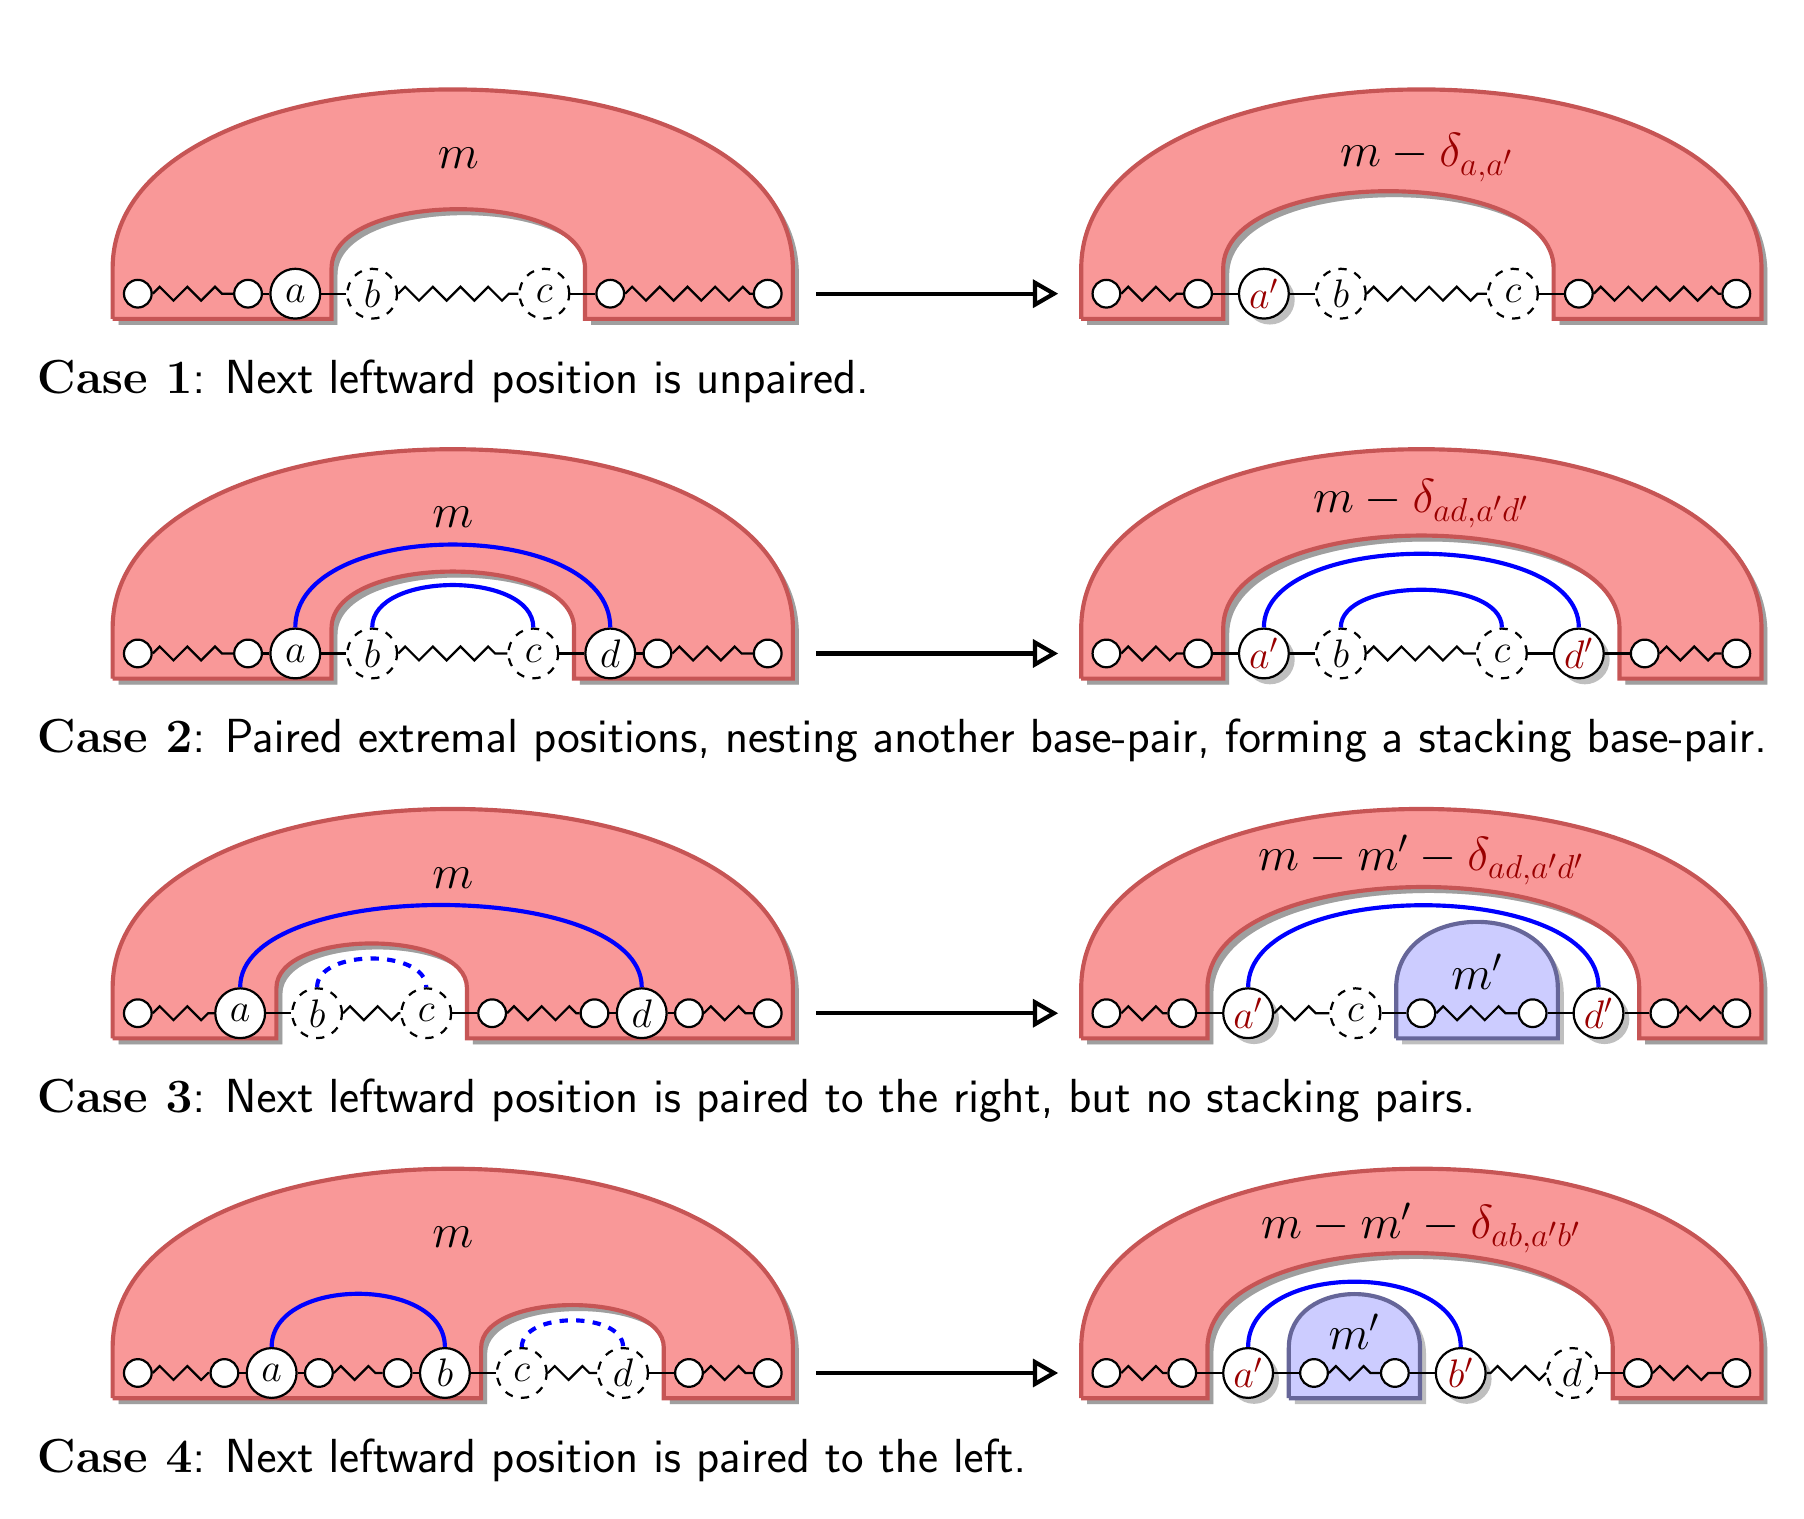
\begin{tikzpicture}
  \definecolor{rougeForb}{HTML}{eb23238f}
  \definecolor{rougeForbP}{HTML}{6d1515ff}

  \newcommand{\BSep}{9pt}
  \newcommand{\HSep}{350pt}
  \newcommand{\RelPosA}{0pt}
  \newcommand{\RelPosB}{-130pt}
  \newcommand{\RelPosC}{-260pt}
  \newcommand{\RelPosD}{-390pt}
  \newcommand{\FitSep}{3.5pt}

  \newcommand{\LabSepB}{15pt}


  \newcommand{\CaptionTxtA}{{\bf Case 1}: Next leftward position is unpaired.}
  \newcommand{\CaptionTxtB}{{\bf Case 2}: Paired extremal positions, nesting another base-pair, forming a stacking base-pair.}
  \newcommand{\CaptionTxtC}{{\bf Case 3}: Next leftward position is paired to the right, but no stacking pairs.}
  \newcommand{\CaptionTxtD}{{\bf Case 4}: Next leftward position is paired to the left.}


  \tikzstyle{caption}=[%fill=gray!20,draw=gray!60,thick,inner sep=4pt,rounded corners=6pt,
font=\relsize{+3}\sffamily,anchor=north west,xshift=-40pt]


  \tikzstyle{basebase}=[circle,draw,thick,inner sep=0,minimum width=18pt,fill=white,font=\relsize{+2}]

  \tikzstyle{base}=[basebase]
  \tikzstyle{basesmall}=[basebase,minimum width=10pt]
  \tikzstyle{basephantom}=[basebase,dashed]
  \tikzstyle{linez}=[draw,snake=zigzag, segment aspect=.2,%
line after snake=0pt,  
        segment length=10pt,thick]
  \tikzstyle{lined}=[linez,draw,snake=none,thick]
  \tikzstyle{line}=[linez,draw,snake=none,thick]
  \tikzstyle{lineh}=[linez]
  \tikzstyle{bp}=[in=90,out=90,draw,line width=1.5pt,blue,looseness=1.7]
  \tikzstyle{blockin}=[trapezium,trapezium angle=83,  fill=blue!20, draw=blue!20!gray,line width=1.5pt, inner sep=0,drop shadow]
  \tikzstyle{blockout}=[blockin,draw=red!80!white!55!gray,fill=red!40!white!95!gray,line width=1.5pt, drop shadow]
  \tikzstyle{lbl}=[inner sep=0,font=\relsize{+3}]
  \tikzstyle{arr}=[-open triangle 60,line width=1.5pt]


 %%%%%%% Unpaired %%%%%%%
  \begin{scope}[yshift=\RelPosA]
 %%%%%%% LHS %%%%%%%
  \begin{scope}[xshift=-\HSep]
  \node[basesmall] (n-beg) at (0,0) {};
  \node[basesmall] (a-0b) at (1.4,0) {};
  \node[base] (a-0) at (2,0) {$a$};
  \node[basesmall] (a-3) at (6,0) {};
  \node[basesmall] (n-end) at (8,0) {};
  \node[right=\BSep of a-0, basephantom] (a-1) {$b$};
  \node[left=\BSep of a-3, basephantom] (a-2) {$c$};
  \path[lineh] (a-1) --  node[lbl,pos=.5,above=45pt] (lbl1) {$m$}  (a-2);
  \path[lined] (a-0) -- (a-1);
  \path[lined] (a-2) -- (a-3);
  \path[linez] (n-beg) -- (a-0b);
  \path[lined] (a-0b) -- (a-0);
  \path[linez] (a-3) -- (n-end);

  \node[right=5pt of n-end] (x) {};



  \begin{pgfonlayer}{background}
  \node[rectangle,inner sep=\FitSep,draw,fit=(n-beg)(a-0.east)] (r1) {};
  \node[rectangle,inner sep=\FitSep,draw,fit=(n-end)(a-3.west)] (r2) {};
  \path[blockout]   (r1.south west) to (r1.south east) to (r1.north east) to[out=90,in=90,looseness=0.8] (r2.north west) to (r2.south west) to (r2.south east) to (r2.north east) to[out=90,in=90,looseness=0.9] (r1.north west) to (r1.south west) ;
  \end{pgfonlayer}{background}

\node[below= \LabSepB of n-beg, caption] {\CaptionTxtA};

  \end{scope}
 %%%%%%% /LHS %%%%%%%



  \node[basesmall] (n-beg) at (0,0) {};
  \node[base, drop shadow] (a-0) at (2,0) {\color{StressColor}$a'$};
  \node[basesmall,left=\BSep of a-0] (a-0b) {};
  \node[basesmall] (a-3) at (6,0) {};
  \node[basesmall] (n-end) at (8,0) {};
  \node[right=\BSep of a-0, basephantom] (a-1) {$b$};
  \node[left=\BSep of a-3, basephantom] (a-2) {$c$};
  \path[lineh] (a-1) --  node[lbl,pos=.5,above=40pt] (lbl1) {$m-{\color{StressColor}\delta_{a,a'}}$}  (a-2);
  \path[lined] (a-0) -- (a-1);
  \path[lined] (a-2) -- (a-3);
  \path[lined] (a-0) -- (a-0b);
  \path[linez] (n-beg) -- (a-0b);
  \path[linez] (a-3) -- (n-end);



  \node[left=5pt of n-beg] (y1) {};

  \path (x) edge[arr]    (y1);

  \begin{pgfonlayer}{background}
  \node[rectangle,inner sep=\FitSep,draw,fit=(n-beg)(a-0b.east)] (r1) {};
  \node[rectangle,inner sep=\FitSep,draw,fit=(n-end)(a-3.west)] (r2) {};
  \path[blockout]   (r1.south west) to (r1.south east) to (r1.north east) to[out=90,in=90,looseness=0.8] (r2.north west) to (r2.south west) to (r2.south east) to (r2.north east) to[out=90,in=90,looseness=0.9] (r1.north west) to (r1.south west) ;
  \end{pgfonlayer}{background}
  \end{scope}



 %%%%%%% /Unpaired %%%%%%%


 %%%%%%% Stacking %%%%%%%
  \begin{scope}[yshift=\RelPosB]

 %%%%%%% LHS %%%%%%%
  \begin{scope}[xshift=-\HSep]
  \node[basesmall] (n-beg) at (0,0) {};
  \node[basesmall] (a-0b) at (1.4,0) {};
  \node[base] (a-0) at (2,0) {$a$};
  \node[base] (a-3) at (6,0) {$d$};
  \node[basesmall] (a-3b) at (6.6,0) {};
  \node[basesmall] (n-end) at (8,0) {};
  \node[right=\BSep of a-0, basephantom] (a-1) {$b$};
  \node[left=\BSep of a-3, basephantom] (a-2) {$c$};
  \path[lineh] (a-1) --  node[lbl,pos=.5,above=45pt] (lbl1) {$m$}  (a-2);
  \path[lined] (a-0) -- (a-1);
  \path[lined] (a-2) -- (a-3);
  \path[linez] (n-beg) -- (a-0b);
  \path[lined] (a-0b) -- (a-0);
  \path[lined] (a-3) -- (a-3b);
  \path[linez] (a-3b) -- (n-end);

  \node[right=5pt of n-end] (x) {};

  \draw[bp,looseness=.9] (a-0) to (a-3);
  \draw[bp,looseness=.9] (a-1) to (a-2);


  \begin{pgfonlayer}{background}
  \node[rectangle,inner sep=\FitSep,draw,fit=(n-beg)(a-0.east)] (r1) {};
  \node[rectangle,inner sep=\FitSep,draw,fit=(n-end)(a-3.west)] (r2) {};
  \path[blockout]   (r1.south west) to (r1.south east) to (r1.north east) to[out=90,in=90,looseness=0.8] (r2.north west) to (r2.south west) to (r2.south east) to (r2.north east) to[out=90,in=90,looseness=0.9] (r1.north west) to (r1.south west) ;
  \end{pgfonlayer}{background}
  \end{scope}

\node[below= \LabSepB of n-beg, caption] {\CaptionTxtB};

 %%%%%%% /LHS %%%%%%%


  \node[basesmall] (n-beg) at (0,0) {};
  \node[base, drop shadow] (a-0) at (2,0) {\color{StressColor}$a'$};
  \node[basesmall,left=\BSep of a-0] (a-0b) {};
  \node[base, drop shadow] (a-3) at (6,0) {\color{StressColor}$d'$};
  \node[basesmall,right=\BSep of a-3] (a-3b) {};
  \node[basesmall] (n-end) at (8,0) {};
  \node[right=\BSep of a-0, basephantom] (a-1) {$b$};
  \node[left=\BSep of a-3, basephantom] (a-2) {$c$};
  \path[lineh] (a-1) --  node[lbl,pos=.5,above=45pt] (lbl1) {$m-{\color{StressColor}\delta_{ad,a'd'}}$}  (a-2);
  \path[lined] (a-0) -- (a-1);
  \path[lined] (a-2) -- (a-3);
  \path[lined] (a-0) -- (a-0b);
  \path[lined] (a-3b) -- (a-3);
  \path[linez] (n-beg) -- (a-0b);
  \path[linez] (a-3b) -- (n-end);
  \draw[bp,looseness=.8] (a-1) to (a-2);
  \draw[bp,looseness=.8] (a-0) to (a-3);




  \node[left=5pt of n-beg] (y2) {};

  \path (x) edge[arr]    (y2);


  \begin{pgfonlayer}{background}
  \node[rectangle,inner sep=\FitSep,draw,fit=(n-beg)(a-0b.east)] (r1) {};
  \node[rectangle,inner sep=\FitSep,draw,fit=(n-end)(a-3b.west) ] (r2) {};
  \path[blockout]   (r1.south west) to (r1.south east) to (r1.north east) to[out=90,in=90,looseness=0.8] (r2.north west) to (r2.south west) to (r2.south east) to (r2.north east) to[out=90,in=90,looseness=0.9] (r1.north west) to (r1.south west) ;
  \end{pgfonlayer}{background}
  \end{scope}
 %%%%%%% /Stacking %%%%%%%

 %%%%%%% BPRight %%%%%%%


  \begin{scope}[yshift=\RelPosC]

 %%%%%%% LHS %%%%%%%
  \begin{scope}[xshift=-\HSep]
  \node[basesmall] (n-beg) at (0,0) {};
  \node[base] (a-0) at (1.3,0) {$a$};
  \node[basesmall] (a-3) at (4.5,0) {};
  \node[basesmall] (a-4b) at (5.8,0) {};
  \node[base] (a-4) at (6.4,0) {$d$};
  \node[basesmall] (a-4t) at (7,0) {};
  \node[basesmall] (n-end) at (8,0) {};
  \node[right=\BSep of a-0, basephantom] (a-1) {$b$};
  \node[left=\BSep of a-3, basephantom] (a-2) {$c$};
  \path (n-beg) --  node[lbl,pos=.5,above=45pt] (lbl1) {$m$}  (n-end);
  \path[lineh] (a-1) --   (a-2);
  \path[lined] (a-0) -- (a-1);
  \path[lined] (a-2) -- (a-3);
  \path[linez] (n-beg) -- (a-0);
  \path[linez] (a-3) -- (a-4b);
  \path[line] (a-4b) -- (a-4);
  \path[line] (a-4) -- (a-4t);
  \path[linez] (a-4t) -- (n-end);

  \draw[bp,looseness=.7] (a-0) to (a-4);
  \draw[bp,looseness=.9,dashed] (a-1) to (a-2);


  \node[right=5pt of n-end] (x) {};

  \begin{pgfonlayer}{background}
  \node[rectangle,inner sep=\FitSep,draw,fit=(n-beg)(a-0.east)] (r1) {};
  \node[rectangle,inner sep=\FitSep,draw,fit=(n-end)(a-3.west) ] (r2) {};
  \path[blockout]   (r1.south west) to (r1.south east) to (r1.north east) to[out=90,in=90,looseness=0.8] (r2.north west) to (r2.south west) to (r2.south east) to (r2.north east) to[out=90,in=90,looseness=0.9] (r1.north west) to (r1.south west) ;
  \end{pgfonlayer}{background}
  \end{scope}

\node[below= \LabSepB of n-beg, caption] {\CaptionTxtC};

 %%%%%%% /LHS %%%%%%%

  \node[basesmall] (n-beg) at (0,0) {};
  \node[base,drop shadow] (a-0) at (1.8,0) {\color{StressColor}$a'$};
  \node[basesmall,left=\BSep of a-0] (a-0b) {};
  \node[base,drop shadow] (a-3) at (6.25,0) {\color{StressColor}$d'$};
  \node[basesmall] (b-1) at (4.0,0) {};
  \node[basesmall,left=\BSep of a-3] (b-2){};
  \node[basesmall,right=\BSep of a-3] (a-3b) {};
  \node[basesmall] (n-end) at (8,0) {};
  %\node[right=\BSep of a-0, basephantom] (a-1) {$a$};
  \node[left=\BSep of b-1, basephantom] (a-2) {$c$};
  \path[lineh] (a-0) --   (a-2);
  \path[lined] (a-2) -- (b-1);
  \path[linez] (b-1) -- node[lbl,pos=.5,above=8pt] (lbl1) {$m'$}  (b-2);
  \path (n-beg) -- node[lbl,pos=.5,above=46pt] (lbl1) {$m-m'-{\color{StressColor}\delta_{ad,a'd'}}$}  (n-end);
  \path[lined] (b-2) -- (a-3);
  \path[lined] (a-0) -- (a-0b);
  \path[lined] (a-3b) -- (a-3);
  \path[linez] (n-beg) -- (a-0b);
  \path[linez] (a-3b) -- (n-end);
  \draw[bp,looseness=.8] (a-0) to (a-3);

  \node[left=5pt of n-beg] (y3) {};
  \path (x) edge[arr]    (y3);

  \begin{pgfonlayer}{background}
  \node[rectangle,inner sep=\FitSep,draw,fit=(n-beg)(a-0b.east)] (r1) {};
  \node[rectangle,inner sep=\FitSep,draw,fit=(n-end)(a-3b.west) ] (r2) {};
  \path[blockout]   (r1.south west) to (r1.south east) to (r1.north east) to[out=90,in=90,looseness=0.8] (r2.north west) to (r2.south west) to (r2.south east) to (r2.north east) to[out=90,in=90,looseness=0.9] (r1.north west) to (r1.south west) ;

  \node[rectangle,inner sep=\FitSep,draw,fit=(b-1)(b-2) ] (r3) {};
  \path[blockin]   (r3.south west) to (r3.south east) to (r3.north east) to[out=90,in=90,looseness=1.4] (r3.north west) to (r3.south west) ;
  \end{pgfonlayer}{background}
  \end{scope}
 %%%%%%% /BPRight %%%%%%%


 %%%%%%% BP Left %%%%%%%
  \begin{scope}[yshift=\RelPosD]

 %%%%%%% LHS %%%%%%%
  \begin{scope}[xshift=-\HSep]
  \node[basesmall] (n-beg) at (0,0) {};
  \node[basesmall] (a-w) at (1.1,0) {};
  \node[base] (a-x) at (1.7,0) {$a$};
  \node[basesmall] (a-y) at (2.3,0) {};
  \node[basesmall] (a-z) at (3.3,0) {};
  \node[base] (a-0) at (3.9,0) {$b$};
  \node[basesmall] (a-3) at (7,0) {};
  \node[basesmall] (n-end) at (8,0) {};
  \node[right=\BSep of a-0, basephantom] (a-1) {$c$};
  \node[left=\BSep of a-3, basephantom] (a-2) {$d$};
  \path[lineh] (a-1) --  (a-2);
  \path (n-beg) --  node[lbl,pos=.5,above=45pt] (lbl1) {$m$}  (n-end);
  \path[lined] (a-0) -- (a-1);
  \path[lined] (a-2) -- (a-3);
  \path[linez] (n-beg) -- (a-w);
  \path[line] (a-w) -- (a-x);
  \path[linez] (a-x) -- (a-y);
  \path[linez] (a-y) -- (a-z);
  \path[line] (a-z) -- (a-0);
  \path[linez] (a-3) -- (n-end);

  \node[right=5pt of n-end] (x) {};

  \draw[bp,looseness=1.05] (a-x) to (a-0);
  \draw[bp,looseness=.9,dashed] (a-1) to (a-2);


  \begin{pgfonlayer}{background}
  \node[rectangle,inner sep=\FitSep,draw,fit=(n-beg)(a-0.east)] (r1) {};
  \node[rectangle,inner sep=\FitSep,draw,fit=(n-end)(a-3.west) ] (r2) {};
  \path[blockout]   (r1.south west) to (r1.south east) to (r1.north east) to[out=90,in=90,looseness=0.8] (r2.north west) to (r2.south west) to (r2.south east) to (r2.north east) to[out=90,in=90,looseness=0.9] (r1.north west) to (r1.south west) ;
  \end{pgfonlayer}{background}
  \end{scope}
 
\node[below= \LabSepB of n-beg, caption] {\CaptionTxtD};


%%%%%%% /LHS %%%%%%%

  \node[basesmall] (n-beg) at (0,0) {};
  \node[base, drop shadow] (a-0) at (1.8,0) {\color{StressColor}$a'$};
  \node[basesmall,left=\BSep of a-0] (a-0b) {};
  \node[base, drop shadow] (a-3) at (4.5,0) {\color{StressColor}$b'$};
  \node[basesmall,right=\BSep of a-0] (b-1)  {};
  \node[basesmall,left=\BSep of a-3] (b-2){};
  \node[basesmall] (a-3b)  at (6.75,0) {};
  \node[basephantom,left=\BSep of a-3b] (a-3c){$d$};
  \node[basesmall] (n-end) at (8,0) {};


  %\node[right=\BSep of a-0, basephantom] (a-1) {$a$};
  %\node[left=\BSep of b-1, basephantom] (a-2) {$b$};
  \path[lined] (b-1) -- (a-0);
  \path[linez] (b-1) -- node[lbl,pos=.5,above=8pt] (lbl1) {$m'$}  (b-2);
  \path (n-beg) -- node[lbl,pos=.5,above=43pt] (lbl1) {$m-m'-{\color{StressColor} \delta_{ab,a'b'}}$}  (n-end);
  \path[lined] (a-3b) -- (a-3c);
  \path[lined] (a-0) -- (a-0b);
  \path[lined] (b-2) -- (a-3);
  \path[lineh] (a-3c) -- (a-3);
  \path[linez] (n-beg) -- (a-0b);
  \path[linez] (a-3b) -- (n-end);
  \draw[bp,looseness=1.05] (a-0) to (a-3);

  \node[left=5pt of n-beg] (y4) {};
  \path (x) edge[arr]    (y4);


  \begin{pgfonlayer}{background}
  \node[rectangle,inner sep=\FitSep,draw,fit=(n-beg)(a-0b.east)] (r1) {};
  \node[rectangle,inner sep=\FitSep,draw,fit=(n-end)(a-3b.west) ] (r2) {};
  \path[blockout]   (r1.south west) to (r1.south east) to (r1.north east) to[out=90,in=90,looseness=0.8] (r2.north west) to (r2.south west) to (r2.south east) to (r2.north east) to[out=90,in=90,looseness=0.9] (r1.north west) to (r1.south west) ;

  \node[rectangle,inner sep=\FitSep,draw,fit=(b-1)(b-2)] (r3) {};
  \path[blockin]   (r3.south west) to (r3.south east) to (r3.north east) to[out=90,in=90,looseness=1.4] (r3.north west) to (r3.south west) ;
  \end{pgfonlayer}{background}
  \end{scope}
 %%%%%%% /BP Left %%%%%%%

\end{tikzpicture}\hspace{1em}
\end{document}